\begin{figure}[H]
	\centering
	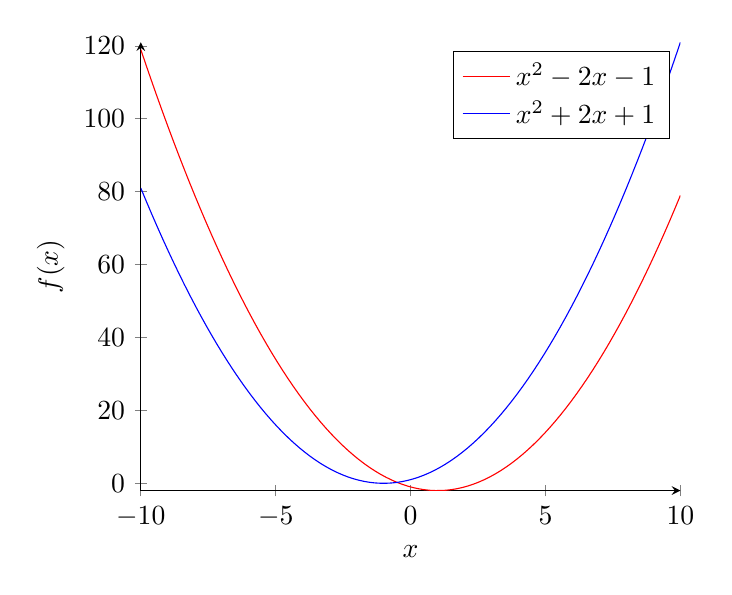
\begin{tikzpicture}
		\begin{axis}[
			axis lines = left,
			xlabel = $x$,
			ylabel = {$f(x)$},
			]
			%Below the red parabola is defined
			\addplot [
			domain=-10:10, 
			samples=100, 
			color=red,
			]
			{x^2 - 2*x - 1};
			\addlegendentry{$x^2 - 2x - 1$}
			%Here the blue parabloa is defined
			\addplot [
			domain=-10:10, 
			samples=100, 
			color=blue,
			]
			{x^2 + 2*x + 1};
			\addlegendentry{$x^2 + 2x + 1$}
		\end{axis}
	\end{tikzpicture}
	\caption{Plot der Funktionen $x^2 - 2x - 1$ und $x^2 + 2x + 1$}
\end{figure}
